%%%
 %
 % Copyright (C) 2019 Ángel Iván Gladín García
 %
 % This program is free software: you can redistribute it and/or modify
 % it under the terms of the GNU General Public License as published by
 % the Free Software Foundation, either version 3 of the License, or
 % (at your option) any later version.
 %
 % This program is distributed in the hope that it will be useful,
 % but WITHOUT ANY WARRANTY; without even the implied warranty of
 % MERCHANTABILITY or FITNESS FOR A PARTICULAR PURPOSE.  See the
 % GNU General Public License for more details.
 %
 % You should have received a copy of the GNU General Public License
 % along with this program.  If not, see <http://www.gnu.org/licenses/>.
%%%

%%%%%%%%%%%%%%%%%%%%%%%%%%%%%%%%%%%%%%%%%%%%%%%%%%%%%%%%%%%%%%%%%%%%%%%%%%%%%%%%%%%%%%%%%
\documentclass[11pt,letterpaper]{report}
\usepackage[margin=1in]{geometry}
\usepackage[utf8]{inputenc}
\usepackage[spanish]{babel}

\usepackage{listings}
\usepackage{color}
\usepackage{graphicx}
\usepackage{enumerate}
\usepackage{enumitem}
\usepackage{float}

\usepackage{longtable}
\usepackage{hyperref}
\usepackage{tikz}

\usepackage{commath}

\usepackage{bbm}
\usepackage{dsfont}
\usepackage{mathrsfs}
\usepackage{amsmath,amsthm,amssymb}
\usepackage{mathtools}
\usepackage{longtable}
%%%%%%%%%%%%%%%%%%%%%%%%%%%%%%%%%%%%%%%%%%%%%%%%%%%%%%%%%%%%%%%%%%%%%%%%%%%%%%%%%%%%%%%%%%%%%%%%5

\usepackage{import}

\usepackage[utf8]{inputenc}

\usepackage{listings}
\usepackage{color}

\definecolor{codegreen}{rgb}{0,0.6,0}
\definecolor{codegray}{rgb}{0.5,0.5,0.5}
\definecolor{codepurple}{rgb}{0.58,0,0.82}
\definecolor{backcolour}{rgb}{0.95,0.95,0.92}

\lstdefinestyle{mystyle}{
    backgroundcolor=\color{backcolour},
    commentstyle=\color{codegreen},
    keywordstyle=\color{magenta},
    numberstyle=\tiny\color{codegray},
    stringstyle=\color{codepurple},
    basicstyle=\footnotesize,
    breakatwhitespace=false,
    breaklines=true,
    captionpos=b,
    keepspaces=true,
    numbers=left,
    numbersep=5pt,
    showspaces=false,
    showstringspaces=false,
    showtabs=false,
    tabsize=2
}

\lstset{style=mystyle}
%%%%%%%%%%%%%%%%%%%%%%%%%%%%%%%%%%%%%%%%%%%%%%%%%%%%%%%%%%%%%%%%%%%%%%%%%%%%%%%%%%%%%%%%%


%%%%%%%%%%%%%%%%%%%%%%%%%%%%%%%%%%%%%%%%%%%%%%%%%%%%%%%%%%%%%%%%%%%%%%%%%%%%%%%%%%%%%%%%%
\newcommand{\Z}{\mathbb{Z}}
\newcommand{\N}{\mathbb{N}}
\newcommand{\Q}{\mathbb{Q}}
\newcommand{\R}{\mathbb{R}}
\newcommand{\Oh}{\mathcal{O}} %% Notacion "O"
\newcommand{\lra}{\longrightarrow}
\newcommand{\ra}{\rightarrow}
\newcommand{\ord}{\text{ord}}
\newcommand{\sol}{\textbf{\underline{Solución}: }} %% Solucion

%%%%%%%%%%%%%%%%%%%%%%%%%%%%%%%%%%%%%%%%%%%%%%%%%%%%%%%%%%%%%%%%%%%%%%%%%%%%%%%%%%%%%%%%%

\usepackage{filecontents}
\begin{filecontents*}{references.bib}
    @book{books/daglib/0072413,
    author = {Papadimitriou, Christos H.},
    keywords = {complexity computational},
    pages = {I-XV, 1-523},
    publisher = {Addison-Wesley},
    timestamp = {2012-03-20T05:17:53.000+0100},
    title = {Computational complexity.},
    year = 1994
    }
    @book{Garey:1979:CIG:578533,
    author = {Garey, Michael R. and Johnson, David S.},
    title = {Computers and Intractability: A Guide to the Theory of NP-Completeness},
    year = {1979},
    isbn = {0716710447},
    publisher = {W. H. Freeman \& Co.},
    address = {New York, NY, USA},
    } 

    @book{papa:COA:31027,
    author = {Papadimitriou, Christos H. and Steiglitz, Kenneth},
    title = {Combinatorial Optimization: Algorithms and Complexity},
    year = {1982},
    isbn = {0-13-152462-3},
    publisher = {Prentice-Hall, Inc.},
    address = {Upper Saddle River, NJ, USA},
    }
    
    @misc{coNPWiki11:online,
    author = {},
    title = {co-NP - Wikipedia},
    howpublished = {\url{https://en.wikipedia.org/wiki/Co-NP}},
    month = {},
    year = {},
    note = {(Accessed on 09/17/2019)}
    }
\end{filecontents*}

\begin{document}

%%%%%%%%%%%%%%%%%%%%%%%%%%%%%%%%%%%%%%%%%%%%%%%%%%%%%%%%%%%%%%%%%%%%%%%%%%%%%%%%%%%%%%%%%
\title{
        Universidad Nacional Autónoma de México\\
        Facultad de Ciencias\\
        Complejidad Computacional\\
    \vspace{1cm}
    \large
        \textbf{Tarea 3}\\
}
\author{
    Ángel Iván Gladín García\\
    No. cuenta: 313112470\\
    \texttt{angelgladin@ciencias.unam.mx}
}
\date{17 de Septiembre 2019}
\maketitle
%%%%%%%%%%%%%%%%%%%%%%%%%%%%%%%%%%%%%%%%%%%%%%%%%%%%%%%%%%%%%%%%%%%%%%%%%%%%%%%%%%%%%%%%%

%%%%%%%%%%%%%%%%%%%%%%%%%%%%%%%%%%%%%%%%%%%%%%%%%%%%%%%%%%%%%%%%%%%%%%%%%%%%%%%%%%%%%%%%%
\newtheorem{theorem}{Teorema}
\newtheorem{example}{Ejemplo}
\newtheorem{corollary}{Corolario}
\newtheorem{lemma}{Lemma}
\newtheorem{definition}{Definicion}
\newtheorem{prop}{Proposicion}
%%%%%%%%%%%%%%%%%%%%%%%%%%%%%%%%%%%%%%%%%%%%%%%%%%%%%%%%%%%%%%%%%%%%%%%%%%%%%%%%%%%%%%%%%


%%%%%%%%%%%%%%%%%%%%%%%%%%%%%%%%%%%%%%%%%%%%%%%%%%%%%%%%%%%%%%%%%%%%%%%%%%%%%%%%%%%%%%%%%
\begin{enumerate}
\item Seleccione \textbf{uno} de los siguientes dos ejerccios:
    \begin{enumerate}
        \item Defina un \emph{programa} \textbf{M} para una MTD que acepte el siguiente lenguaje:
        \[
            \mathscr{L} = \{ 0(0+1)^*0 + 1(0+1)^*1 \}
        \]

        Lo primero que se hará por cuestiones de facilidad es crear un autómata finito
        no determinista \emph{(NFA)} y después pasarlo a una MTD.
        \begin{center}
            \begin{tikzpicture}[scale=0.2]
            \tikzstyle{every node}+=[inner sep=0pt]
            \draw [black] (11.7,-21.6) circle (3);
            \draw (11.7,-21.6) node {$q_0$};
            \draw [black] (28.7,-13.7) circle (3);
            \draw (28.7,-13.7) node {$q_1$};
            \draw [black] (29.3,-28.3) circle (3);
            \draw (29.3,-28.3) node {$q_2$};
            \draw [black] (45.7,-13.7) circle (3);
            \draw (45.7,-13.7) node {$q_3$};
            \draw [black] (45.7,-13.7) circle (2.4);
            \draw [black] (45.7,-28.3) circle (3);
            \draw (45.7,-28.3) node {$q_4$};
            \draw [black] (45.7,-28.3) circle (2.4);
            \draw [black] (4.4,-21.6) -- (8.7,-21.6);
            \fill [black] (8.7,-21.6) -- (7.9,-21.1) -- (7.9,-22.1);
            \draw [black] (14.5,-22.67) -- (26.5,-27.23);
            \fill [black] (26.5,-27.23) -- (25.93,-26.48) -- (25.57,-27.42);
            \draw (19.56,-25.47) node [below] {$0$};
            \draw [black] (14.42,-20.34) -- (25.98,-14.96);
            \fill [black] (25.98,-14.96) -- (25.04,-14.85) -- (25.46,-15.75);
            \draw (19.22,-17.14) node [above] {$1$};
            \draw [black] (27.377,-11.02) arc (234:-54:2.25);
            \draw (28.7,-6.45) node [above] {$1$};
            \fill [black] (30.02,-11.02) -- (30.9,-10.67) -- (30.09,-10.08);
            \draw [black] (30.623,-30.98) arc (54:-234:2.25);
            \draw (29.3,-35.55) node [below] {$0$};
            \fill [black] (27.98,-30.98) -- (27.1,-31.33) -- (27.91,-31.92);
            \draw [black] (30.865,-11.637) arc (125.71019:54.28981:10.854);
            \fill [black] (43.54,-11.64) -- (43.18,-10.76) -- (42.59,-11.58);
            \draw (37.2,-9.1) node [above] {$0$};
            \draw [black] (43.271,-15.448) arc (-61.10225:-118.89775:12.562);
            \fill [black] (31.13,-15.45) -- (31.59,-16.27) -- (32.07,-15.4);
            \draw (37.2,-17.51) node [below] {$0,1$};
            \draw [black] (31.728,-26.552) arc (118.61949:61.38051:12.05);
            \fill [black] (43.27,-26.55) -- (42.81,-25.73) -- (42.33,-26.61);
            \draw (37.5,-24.58) node [above] {$1$};
            \draw [black] (43.236,-29.999) arc (-62.35949:-117.64051:12.365);
            \fill [black] (31.76,-30) -- (32.24,-30.81) -- (32.7,-29.93);
            \draw (37.5,-31.91) node [below] {$1,0$};
            \end{tikzpicture}
            \end{center}
            
            Recordando la definición de MT que es:
            $$M = (Q, \Sigma, \Gamma, \delta, s, B, F)$$

            Donde tenemos que:
            \begin{itemize}
                \item $Q = \{ q_0, q_1, q_2, q_3, q_4\}$
                \item $\Sigma = \{ 0, 1 \}$
                \item $\Gamma = \{ 0, 1, \# \}$
                \item $\delta$ dada por:
                \begin{table}[H]
                    \centering
                    \begin{tabular}{|l|l|l|l|}
                    \hline
                    Estado & 0 & 1 & $\#$ \\ \hline
                    $q_0$ & $(q_1, 1, R)$ & $(q_2, 1, R)$ & $-$ \\ \hline
                    $q_1$ & $(q_3, 0, R)$ & $(q_1, 1, R)$ & $-$ \\ \hline
                    $q_2$ & $(q_2, 0, R)$ & $(q_4, 1, R)$ & $-$ \\ \hline
                    $q_3$ & $(q_1, 0, R)$ & $(q_1, 1, R)$ & $(q_3, \#, R)$ \\ \hline
                    $q_4$ & $(q_2, 0, R)$ & $(q_2, 1, R)$ & $(q_4, \#, R)$ \\ \hline
                    \end{tabular}
                \end{table}
                \item $s = q_0$
                \item $B = \#$
                \item $F = \{ q_3, q_4 \}$
            \end{itemize}

        \item Defina un \emph{programa} \textbf{M} para una MTD que acepte el siguiente lenguaje:
        \[
            \mathscr{L} = \{ 1^n0^m | n,m \geq 0 \land 2 | (n+m) \}
        \]
        \textbf{Hint:}
        \[
            \mathscr{L} = \{ (11)^*(00)^* + 1(11)^*0(00)^* \}    
        \]
    \end{enumerate}

\item Definir formalmente, en términos de problemas y en términos de lenguajes, las clases:
\begin{itemize}
    \item \textit{CoP}
    \begin{itemize}
        \item En términos de problemas:
        $$\text{co-P} = \{ \Pi^c : \Pi \in P \}$$

        \item En términos de lenguajes:
        
        Sea $\Pi$ un problema en $P$ codificado en un alfabeto $\Sigma$ y decimos que hay una cadena
        $s$ que es aceptado, por otro lado, sea $\Pi^c$ un problema en $P$ decimos que hay una
        cadena $w$ que es aceptada.
    \end{itemize}
    

    \item \textit{CoNP}
    \begin{itemize}
        \item En términos de problemas:
        $$\text{co-NP} = \{ \Pi^c : \Pi \in NP \}$$

        \item En términos de lenguajes:
        $$\text{co-NP} = \{ \Sigma^* - L : L \text{ es es una lenguaje sobre el alfabeto $\Sigma$ 
        y } L \in NP \}$$
    \end{itemize}
    
\end{itemize}


\item Seleccionar dos de los siguientes problemas en la clase \textbf{P}, plantearlos como problemas
de decisión y enunciar sus complementos.
\begin{itemize}
    \item Problema Flujo Máximo

    \item Problema de Ruta más corta.
    
    \textbf{Ejemplar:} Dada un gráfica $G=(V,E)$, un peso en cada arista $w(e)$, y un número $k$.\\
    \textbf{Pregunta:} ¿Existe un camino de $u$ a $v$ de a lo más $k$ (la suma del peso de sus aristas)?
    
    \medskip
    \textbf{Complemento:}\\
    \textbf{Ejemplar:} Dada un gráfica $G=(V,E)$, un peso en cada arista $w(e)$, y un número $k$.\\
    \textbf{Pregunta:} ¿Para todo camino de $u$ a $v$ es mayor que $k$?

    \item Problema Apareamiento en gráficas bipartitas
    
    \textbf{Ejemplar:} Dada una gráfica bipartita $G = (U,V,E)$, un apareamiento $M$ y un número $k$.\\
    \textbf{Pregunta:} ¿Existe un apareamiento bipartito que sea por lo menos de tamaño $k$?

    \medskip
    \textbf{Complemento:}\\
    \textbf{Ejemplar:} Dada una gráfica bipartita $G = (U,V,E)$, un apareamiento $M$ y un número $k$.\\
    \textbf{Pregunta:} ¿Para todo apareamiento bipartito es de tamaño menor a $k$?
\end{itemize}



\item Seleccionar dos de los siguientes problemas en la clase \textbf{NP}, plantearlos como
problemas de decisión y enunciar sus complementos.
\begin{itemize}
    \item Problema de Coloración en Gráficas.
    

    \item Problema del Clan:
    
    \textbf{Ejemplar:} Gráfica $G$, entero positivo $K$.\\
    \textbf{Pregunta:} ¿La subgráfica completa más grande en $G$ contiene exactamente 
    $K$ vértices?

    \medskip
    \textbf{Complemento:}\\
    \textbf{Ejemplar:} Gráfica $G$, entero positivo $K$.\\
    \textbf{Pregunta:} ¿$K$ es el tamaño del clan máximo?
    

    \item Problema Conjunto Independiente
    
    \textbf{Ejemplar:} Sea una gráfica $G=(V,E)$ no dirigida y sea $I \subseteq V$. Decimps que $I$
    es un conjunto independiente si cualesquirra $i,j \in I$ entonces no hya una arista entre $i$ y
    $j$\\
    \textbf{Pregunta:} Sea una gráfica $G=(V,E)$ no dirigida y una meta $k$, ¿hay un
    conjunto independiente $I$ con $|I| = k$?

    
    \medskip
    \textbf{Complemento:}\\
    \textbf{Ejemplar:} Sea una gráfica $G=(V,E)$ y un entero positivo $k \leq |V|$.\\
    \textbf{Pregunta:} (De hecho el complemento del conjunto independiente es \emph{Vertex cover}).\\
    Existe una cubierta de vértices de tamaño $k$ o menor para $G$, es decir, un subconjunto $V' \subseteq V$ tal que
    $|V'| \leq k$ y, que para arista $\{u,v\} \in E$, al menos una de $u$ y $v$ pertenezca a $V'$?

\end{itemize}


\item Para uno de los problemas presentados en el ejercicio 3, digamos $\Pi$, muestre que tanto 
$\Pi$ como $\Pi^c$ están en P.

¿Siempre sucede esto? Es decir, \textit{¿P = CoP?} Demuestre.

Primero se revisará el Teorema 16.1\cite{papa:COA:31027}, que dice que si un problema $A$ es un problema en $P$, entonces
el complemento $\bar{A}$ de $A$ está también en $P$.
\begin{proof}
    Como $A$ está en $P$, entonces hay un algoritmo polinomial que resuelve $A$. Un algoritmo
    polinomial para resolver el complemento de $A$ es exactamente el mismo algoritmo, solo con la
    substitución de un \emph{no} en vez de un \emph{sí} cuando fue reportado, y viceversa.
\end{proof}


\item ¿La intersección de \textit{NP} y \textit{coNP} es vacía? Justifica tu respuesta.

\begin{figure}[H]
    \centering
    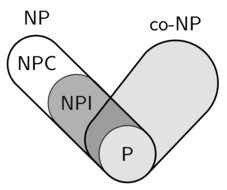
\includegraphics[scale=0.75]{1.png}
    \caption{La intersección no es vacía}
\end{figure}

Por que los problemas \textit{P} están en la intersección de ambos.


\item Ejercicio Adicional (Puntos Adicionales)
\textit{¿NP = coNP?} ¿Quién está contenido en cuál? Justifica tu respuesta.

Como todos los problemas en \textit{NP} pueden ser reducidos a un problema de desición, se sigue que
para cada problema en \textit{NP} podemos construir una máquina de Turing no determinista que decide
su complemento en tiempo polinomial, es decir, \textit{NP} $\subseteq$ \textit{coNP}. De esto se
sigue que que el conjunto de complemento de problemas en \textit{coNP}, es decir,
\textit{coNP} $\subseteq$ \textit{NP}. Por lo tanto \textit{coNP} $=$ \textit{NP}. La prueba de que 
ningun problema \textit{coNP} pueda estar en \textit{NP} si \textit{NP} $\not =$ \textit{coNP} e
simétrica.

\end{enumerate}

%%%%%%%%%%%%%%%%%%%%%%%%%%%%%%%%%%%%%%%%%%%%%%%%%%%%%%%%%%%%%%%%%%%%%%%%%%%%%%%%%%%%%%%%%
\nocite{*}


\bibliographystyle{plain}
\bibliography{references}

%%%%%%%%%%%%%%%%%%%%%%%%%%%%%%%%%%%%%%%%%%%%%%%%%%%%%%%%%%%%%%%%%%%%%%%%%%%%%%%%%%%%%%%%%



%%%%%%%%%%%%%%%%%%%%%%%%%%%%%%%%%%%%%%%%%%%%%%%%%%%%%%%%%%%%%%%%%%%%%%%%%%%%%%%%%%%%%%%%%

\end{document}